\section{Australia model (model ID: 19)}
The Australia model (fig.~\ref{fig:19_schematic}) is part of a top-down modelling exercise (originally referred to as model S4) designed to use auxiliary data \citep{Farmer2003}. 
Some adjustments were made to the evaporation equations: these were originally separated between vegetation and bare soil evaporation, scaled between the unsaturated and saturated zone. 
This has been simplified to separation between unsaturated and saturated evaporation only. 
The model has 3 stores and 8 parameters ($S_b$, $\phi$, $fc$, $\alpha_{SS}$, $\beta_{SS}$, $K_{deep}$,  $\alpha_{BF}$ and $\beta_{BF}$). 
For consistency with other model formulations, $S_b$ is is used as a parameter, instead of being broken down into its constitutive parts $D$ and $\phi$. 
The model aims to represent:

\begin{itemizecompact}
\item Separation of saturated zone and a variable-size unsaturated zone;
\item Evaporation from unsaturated and saturated zones;
\item Saturation excess and non-linear subsurface flow;
\item Deep groundwater recharge and baseflow.
\end{itemizecompact}

\subsection{MARRMoT model name}
m\_19\_australia\_8p\_3s \\

% Equations
\subsection{Model equations}

% Model layout figure
{ 																	% This ensures it doesn't warp text further down
\begin{wrapfigure}{l}{5cm}
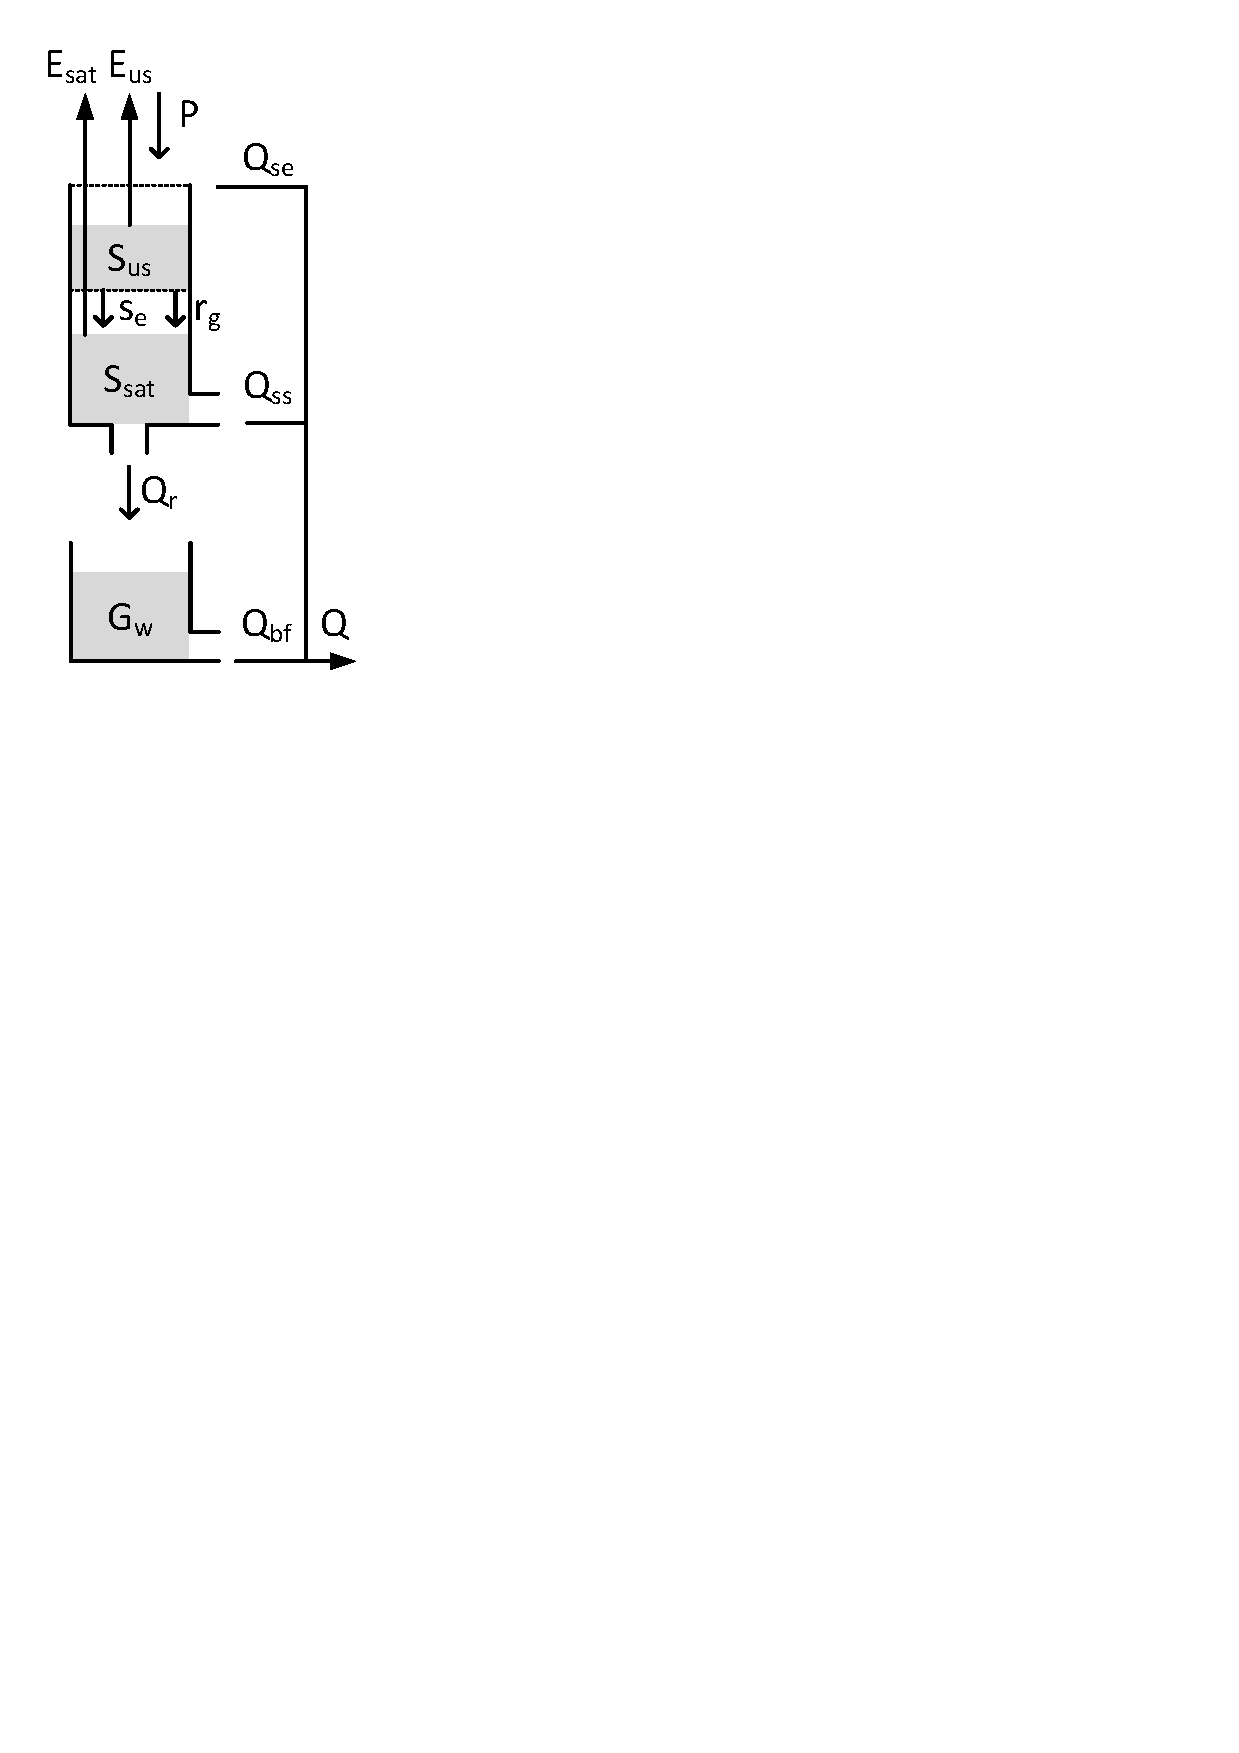
\includegraphics[trim=1cm 18cm 14cm 0.8cm,width=5cm,keepaspectratio]{./AppA_files/19_schematic.pdf}
\caption{Structure of the Australia model} \label{fig:19_schematic}
\end{wrapfigure}

\begin{align}
	\frac{dS_{us}}{dt} &= P-E_{us}-r_g -s_e\\
	E_{us} &= \frac{S_{us}}{S_b}*E_p\\
	S_b &= D*\phi\\
	r_g &= 
	\begin{cases}
		P, & if~S_{us} > S_{usfc}\\
		0, & \text{otherwise} \\
	\end{cases} \\
	s_e &= \begin{cases}
			S_{us} - S_{usfc}, & if~S_{us} > S_{usfc}\\
			0, & \text{otherwise} \\
			\end{cases}\\
	S_{usfc} &= (S_b - S_{sat})*\frac{fc}{\phi} 
\end{align}

Where $S_{us}$ is the current storage in the unsaturated store [mm], $P$ the current precipitation $[mm/d]$, $S_b$ [mm] the maximum storage of the soil profile, based on the soil depth $D$ [mm] and the porosity $\phi$ [-]. $r_g$ $[mm/d]$ is drainage from the unsaturated store to the saturated store, based on the variable field capacity $S_{usfc}$ [mm]. $S_{usfc}$ is based on the current storage on the saturated zone $S_{sat}$ [mm], the maximum soil moisture storage $S_b$ [mm], the field capacity $fc$ [-] and the porosity $\phi$ [-]. $s_e$ $[mm/d]$ is the storage excess, resulting from a decrease of $S_{usfc}$ that leads to more water being stored in the unsaturated zone than should be possible.

} % end wrap

\begin{align}
	\frac{dS_{sat}}{dt} &= r_g - E_{sat} - Q_{SE} - Q_{SS} - Q_{R}\\
	E_{sat} &= \frac{S_{sat}}{S_b}*E_p\\
	Q_{SE} &= \begin{cases}
		r_g+S_e, &\text{if } S_{sat} > S_b \\
		0, & \text{otherwise} \\
	\end{cases} \\
	Q_{SS} &= \alpha_{SS}*\left(S_{sat}\right)^{\beta_{SS}}\\
	Q_{R} &= K_{deep}*S_{sat}
\end{align}

Where $S_{sat}$ is the current storage in the saturated zone [mm], $E_{sat}$ is the evaporation from the saturated zone [mm], $Q_{SE}$ saturation excess runoff $[mm/d]$ that occurs when the saturated zone reaches maximum capacity $S_b$ [mm], $Q_{SS}$ is subsurface flow $[mm/d]$ and $Q_R$ is recharge of deep groundwater $[mm/d]$. Both $Q_{SS}$ and $Q_R$ are based on the dimensionless fraction $r$ and subsurface flow constants $c$ $[d^{-1}]$ and $d$ [-]. 

\begin{align}
	\frac{dG_w}{dt} &= Q_{R} - Q_{BF}\\
	Q_{BF} &= \alpha_{BF}*\left(G_w\right)^{\beta_{BF}}\\
\end{align}

Where $G_w$ is the current groundwater storage [mm] and $Q_{BF}$ baseflow, dependent on parameters  $\alpha_{BF}$ $[d^{-1}]$ and $\beta_{BF}$ [-]. Total runoff is the sum of $Q{SE}$, $Q_{SS}$ and $Q_{BF}$:

\begin{align}
	Q &= Q_{SE} + Q_{SS} + Q_{BF}
\end{align}

\newpage
\subsection{Parameter overview}
% Table generated by Excel2LaTeX from sheet 'Sheet1'
\begin{table}[htbp]
  \centering
    \begin{tabular}{lll}
    \toprule
    Parameter & Unit  & Description \\
    \midrule
    $S_b$ & $mm$  & Maximum soil moisture storage \\
    $\phi$ & $-$   & Porosity \\
    $fc$  & $-$   & Field capacity \\
    $\alpha_{SS}$ & $d^{-1}$ & Runoff coefficient \\
    $\beta_{SS}$ & $-$   & Runoff nonlinearity \\
    $K_{deep}$ & $d^{-1}$ & Runoff coefficient \\
    $\alpha_{BF}$ & $d^{-1}$ & Runoff coefficient \\
    $\beta_{BF}$ & $-$   & Runoff nonlinearity \\
    \bottomrule
    \end{tabular}%
  \label{tab:addlabel}%
\end{table}%

